% questions.tex —— 2002 年·北京卷·文科 · 题目内容片段（无答案）
% 由 tools/generate_projects.py 依来源总账自 2002/2002_数学真题_北京文_试题.md 生成，勿手改（改源 MD 后重跑）


\begin{gktip}
来源说明：本稿按固定来源 PDF 第 1–2 页（印刷页 102–103）转录；题签、页数及 SHA-256 与来源清单一致。固定文件为 ready，但尚无证据将其绑定到具体上游出版物/版次，故保留未绑定状态（卷 ID 置空）。题面中可辨认的原印疑点照录，不据常见题型改字。该 PDF 未见答案页，官方答案字段保持为空。

图形说明：Q4、Q11、Q12、Q18 的 TikZ 图稿及 Q20 两张计算表已由主会话和独立复核者对照固定源页核查。图稿只表达源图可辨认的拓扑、标签和关系，不宣称按比例测绘；Q18 原图未画出题干所述 E、F 延长交点，故不擅自补画。Q19 源内数列记作 $\{a_n\}$ 而元素写作 $x_n$，符号混用照录；Q18「侧棱延长后相交于 $E,F$ 两点」为原印表述，未限定各侧棱归属，照录不补。
\end{gktip}

\gkpart{一、选择题}

\begin{question}
\gkti{1}满足条件 \(M\cup\{1\}=\{1,2,3\}\) 的集合 \(M\) 的个数是\mbox{（　　）}。

（A）4　　（B）3　　（C）2　　（D）1

\end{question}
\begin{question}
\gkti{2}在平面直角坐标系中，已知两点 \(A(\cos80^\circ,\sin80^\circ)\)，\(B(\cos20^\circ,\sin20^\circ)\)，则 \(|AB|\) 的值是\mbox{（　　）}。

（A）\(\dfrac12\)　　（B）\(\dfrac{\sqrt2}{2}\)　　（C）\(\dfrac{\sqrt3}{2}\)　　（D）1

\end{question}
\begin{question}
\gkti{3}下列四个函数中，以 \(\pi\) 为最小正周期，且在区间 \(\left(\dfrac\pi2,\pi\right)\) 上为减函数的是\mbox{（　　）}。

（A）\(y=\cos x\)　　（B）\(y=2|\sin x|\)　　（C）\(y=\cos\dfrac{x}{2}\)　　（D）\(y=-\cot x\)

\Needspace{0.4\textheight}
\end{question}
\begin{question}
\gkti{4}在下列四个正方体中，能得出 \(AB\perp CD\) 的是\mbox{（　　）}。
\nopagebreak[4]
\begin{center}% Reconstructed cube options: preserve the printed vertex and line incidence,
% but do not infer metric proportions from the perspective drawing.
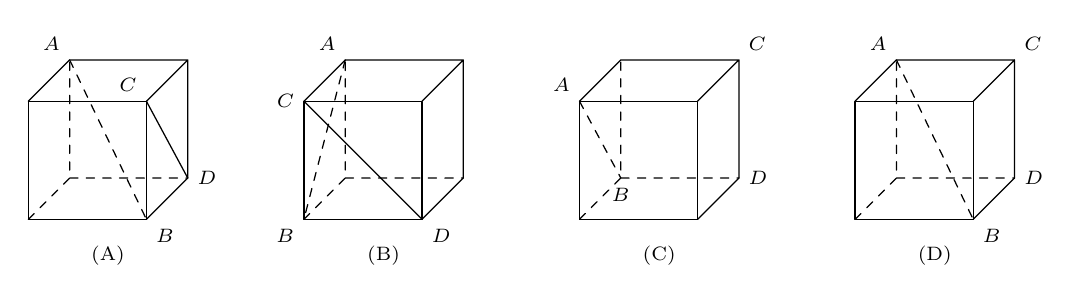
\begin{tikzpicture}[x=.75cm,y=.75cm,line cap=round,line join=round]
\tikzset{cube edge/.style={line width=.45pt}, hidden edge/.style={cube edge,dashed}}

% (A): A=back TL, C=front TR, B=front BR, D=back BR.
\begin{scope}
  \coordinate (a) at (0,0); \coordinate (b) at (2,0);
  \coordinate (c) at (2,2); \coordinate (d) at (0,2);
  \coordinate (e) at (.7,.7); \coordinate (f) at (2.7,.7);
  \coordinate (g) at (2.7,2.7); \coordinate (h) at (.7,2.7);
  \draw[cube edge] (a)--(b)--(c)--(d)--cycle;
  \draw[cube edge] (d)--(h)--(g)--(c) (g)--(f)--(b);
  \draw[hidden edge] (a)--(e)--(h) (e)--(f);
  \draw[hidden edge] (h)--(b);
  \draw[cube edge] (c)--(f);
  \node[font=\scriptsize,above left] at (h) {$A$};
  \node[font=\scriptsize,above left] at (c) {$C$};
  \node[font=\scriptsize,below right] at (b) {$B$};
  \node[font=\scriptsize,right] at (f) {$D$};
  \node[font=\scriptsize] at (1.35,-.62) {(A)};
\end{scope}

% (B): A=back TL, C=front TL, B=front BL, D=front BR.
\begin{scope}[xshift=3.5cm]
  \coordinate (a) at (0,0); \coordinate (b) at (2,0);
  \coordinate (c) at (2,2); \coordinate (d) at (0,2);
  \coordinate (e) at (.7,.7); \coordinate (f) at (2.7,.7);
  \coordinate (g) at (2.7,2.7); \coordinate (h) at (.7,2.7);
  \draw[cube edge] (a)--(b)--(c)--(d)--cycle;
  \draw[cube edge] (d)--(h)--(g)--(c) (g)--(f)--(b);
  \draw[hidden edge] (a)--(e)--(h) (e)--(f);
  \draw[hidden edge] (h)--(a);
  \draw[cube edge] (d)--(b);
  \node[font=\scriptsize,above left] at (h) {$A$};
  \node[font=\scriptsize,left] at (d) {$C$};
  \node[font=\scriptsize,below left] at (a) {$B$};
  \node[font=\scriptsize,below right] at (b) {$D$};
  \node[font=\scriptsize] at (1.35,-.62) {(B)};
\end{scope}

% (C): A=front TL, C=back TR, B=back BL, D=back BR.
\begin{scope}[xshift=7cm]
  \coordinate (a) at (0,0); \coordinate (b) at (2,0);
  \coordinate (c) at (2,2); \coordinate (d) at (0,2);
  \coordinate (e) at (.7,.7); \coordinate (f) at (2.7,.7);
  \coordinate (g) at (2.7,2.7); \coordinate (h) at (.7,2.7);
  \draw[cube edge] (a)--(b)--(c)--(d)--cycle;
  \draw[cube edge] (d)--(h)--(g)--(c) (g)--(f)--(b);
  \draw[hidden edge] (a)--(e)--(h) (e)--(f);
  \draw[hidden edge] (d)--(e);
  \node[font=\scriptsize,above left] at (d) {$A$};
  \node[font=\scriptsize,above right] at (g) {$C$};
  \node[font=\scriptsize,below] at (e) {$B$};
  \node[font=\scriptsize,right] at (f) {$D$};
  \node[font=\scriptsize] at (1.35,-.62) {(C)};
\end{scope}

% (D): A=back TL, C=back TR, B=front BR, D=back BR.
\begin{scope}[xshift=10.5cm]
  \coordinate (a) at (0,0); \coordinate (b) at (2,0);
  \coordinate (c) at (2,2); \coordinate (d) at (0,2);
  \coordinate (e) at (.7,.7); \coordinate (f) at (2.7,.7);
  \coordinate (g) at (2.7,2.7); \coordinate (h) at (.7,2.7);
  \draw[cube edge] (a)--(b)--(c)--(d)--cycle;
  \draw[cube edge] (d)--(h)--(g)--(c) (g)--(f)--(b);
  \draw[hidden edge] (a)--(e)--(h) (e)--(f);
  \draw[hidden edge] (h)--(b);
  \draw[cube edge] (g)--(f);
  \node[font=\scriptsize,above left] at (h) {$A$};
  \node[font=\scriptsize,above right] at (g) {$C$};
  \node[font=\scriptsize,below right] at (b) {$B$};
  \node[font=\scriptsize,right] at (f) {$D$};
  \node[font=\scriptsize] at (1.35,-.62) {(D)};
\end{scope}
\end{tikzpicture}
\end{center}
\nopagebreak[4]
\end{question}
\begin{question}
\gkti{5}64 个直径都为 \(\dfrac a4\) 的球，记它们的体积之和为 \(V_{\text{甲}}\)，表面积之和为 \(S_{\text{甲}}\)；一个直径为 \(a\) 的球，记其体积为 \(V_{\text{乙}}\)，表面积为 \(S_{\text{乙}}\)，则\mbox{（　　）}。

（A）\(V_{\text{甲}}>V_{\text{乙}},\ S_{\text{甲}}>S_{\text{乙}}\)　　（B）\(V_{\text{甲}}<V_{\text{乙}},\ S_{\text{甲}}<S_{\text{乙}}\)

（C）\(V_{\text{甲}}=V_{\text{乙}},\ S_{\text{甲}}>S_{\text{乙}}\)　　（D）\(V_{\text{甲}}=V_{\text{乙}},\ S_{\text{甲}}=S_{\text{乙}}\)

\end{question}
\begin{question}
\gkti{6}若直线 \(l:y=kx-\sqrt3\) 与直线 \(2x+3y-6=0\) 的交点位于第一象限，则直线 \(l\) 的倾斜角的取值范围是\mbox{（　　）}。

（A）\(\left[\dfrac\pi6,\dfrac\pi3\right)\)　　（B）\(\left(\dfrac\pi6,\dfrac\pi2\right)\)

（C）\(\left(\dfrac\pi3,\dfrac\pi2\right)\)　　（D）\(\left[\dfrac\pi6,\dfrac\pi2\right]\)

\end{question}
\begin{question}
\gkti{7}\((1+i)^8\) 等于\mbox{（　　）}。

（A）\(16i\)　　（B）\(-16i\)　　（C）\(-16\)　　（D）16

\end{question}
\begin{question}
\gkti{8}若 \(\dfrac{\cot\theta-1}{2\cot\theta+1}=1\)，则 \(\cos2\theta\) 的值为\mbox{（　　）}。

（A）\(\dfrac{3}{5}\)　　（B）\(-\dfrac{3}{5}\)　　（C）\(\dfrac{2\sqrt5}{5}\)　　（D）\(-\dfrac{2\sqrt5}{5}\)

\end{question}
\begin{question}
\gkti{9}5 本不同的书，全部分给四个学生，每个学生至少 1 本，则不同的分法的种数为\mbox{（　　）}。

（A）480　　（B）240　　（C）120　　（D）96

\end{question}
\begin{question}
\gkti{10}已知椭圆 \(\dfrac{x^2}{3m^2}+\dfrac{y^2}{5n^2}=1\) 和双曲线 \(\dfrac{x^2}{2m^2}-\dfrac{y^2}{3n^2}=1\) 有公共的焦点，那么双曲线的渐近线方程是\mbox{（　　）}。

（A）\(x=\pm\dfrac{\sqrt{15}}2y\)　　（B）\(y=\pm\dfrac{\sqrt{15}}2x\)

（C）\(x=\pm\dfrac{\sqrt3}{4}y\)　　（D）\(y=\pm\dfrac{\sqrt3}{4}x\)

\Needspace{0.4\textheight}
\end{question}
\begin{question}
\gkti{11}已知 \(f(x)\) 是定义在 \((0,3)\) 上的函数，\(f(x)\) 的图象如图所示，那么不等式 \(f(x)\cos x<0\) 的解集是\mbox{（　　）}。
\nopagebreak[4]
\begin{center}% Qualitative reconstruction of the printed function graph on (0,3).
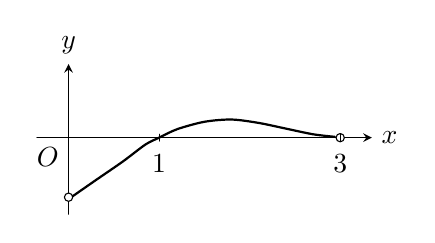
\begin{tikzpicture}[x=1.15cm,y=.72cm,>=stealth,line cap=round,line join=round]
  \draw[->] (-.35,0)--(3.35,0) node[right] {$x$};
  \draw[->] (0,-1.35)--(0,1.3) node[above] {$y$};
  \draw[thick] plot[smooth] coordinates {(.03,-1.05) (.30,-.75) (.60,-.42) (.85,-.12) (1.00,0) (1.20,.15) (1.50,.28) (1.80,.32) (2.10,.26) (2.40,.16) (2.70,.06) (2.94,.015)};
  \draw[fill=white] (0,-1.05) circle (1.5pt);
  \draw[fill=white] (3,0) circle (1.5pt);
  \draw (1,-.06)--(1,.06) node[below=4pt] {$1$};
  \draw (3,-.06)--(3,.06) node[below=4pt] {$3$};
  \node[below left] at (0,0) {$O$};
\end{tikzpicture}
\end{center}
\nopagebreak[4]
（A）\((0,1)\cup(2,3)\)　　（B）\((1,\dfrac\pi2)\cup(\dfrac\pi2,3)\)　　（C）\((0,1)\cup(\dfrac\pi2,3)\)　　（D）\((0,1)\cup(1,3)\)

\Needspace{0.4\textheight}
\end{question}
\begin{question}
\gkti{12}如图所示，\(f_1(x),f_2(x),f_3(x),f_4(x)\) 是定义在 \([0,1]\) 上的四个函数，其中满足性质“对 \([0,1]\) 中任意的 \(x_1\) 和 \(x_2\)，\(f\left(\dfrac{x_1+x_2}{2}\right)\leqslant\dfrac12[f(x_1)+f(x_2)]\) 恒成立”的只有\mbox{（　　）}。
\nopagebreak[4]
\begin{center}% 第 12 题四幅函数图象的结构示意（源图只表示定性形态与端点；比例不作数学条件）。
% 虚线为 x=1 处辅助线，仅 f_2、f_3、f_4 面板有（与源图一致），高度取各自端点值。
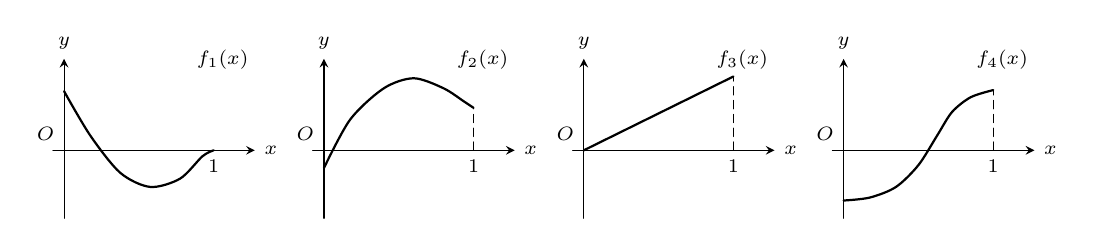
\begin{tikzpicture}[x=.95cm,y=.75cm,>=stealth,line cap=round,line join=round,
  every node/.style={font=\scriptsize}]
\foreach \shift/\name in {0/{f_1(x)},3.3/{f_2(x)},6.6/{f_3(x)},9.9/{f_4(x)}} {
  \begin{scope}[xshift=\shift cm]
    \draw[->] (-.15,0)--(2.55,0) node[right] {$x$};
    \draw[->] (0,-1.15)--(0,1.55) node[above] {$y$};
    \node[above left] at (0,0) {$O$};
    \node[above] at (2.12,1.2) {$\name$};
    \node[below] at (2,0) {$1$};
  \end{scope}
}
% f_1：下凸（碗形），无 x=1 辅助虚线。
\begin{scope}
  \draw[thick] plot[smooth] coordinates {(0,1.0) (.35,.25) (.75,-.38) (1.15,-.62) (1.55,-.48) (1.85,-.10) (2,0)};
\end{scope}
% f_2：上凸（拱形），端点在 x=1 且属于 [0,1]。
\begin{scope}[xshift=3.3cm]
  \draw[thick] plot[smooth] coordinates {(0,-.3) (.35,.52) (.8,1.05) (1.2,1.22) (1.6,1.05) (1.88,.82) (2,.72)};
  \draw[densely dashed] (2,0)--(2,.72);
\end{scope}
% f_3：从原点到右端点的线段。
\begin{scope}[xshift=6.6cm]
  \draw[thick] (0,0)--(2,1.25);
  \draw[densely dashed] (2,0)--(2,1.25);
\end{scope}
% f_4：S-shaped curve with a change of concavity，仅示意。
\begin{scope}[xshift=9.9cm]
  \draw[thick] plot[smooth] coordinates {(0,-.85) (.35,-.8) (.7,-.62) (1,-.25) (1.25,.25) (1.45,.65) (1.7,.9) (2,1.02)};
  \draw[densely dashed] (2,0)--(2,1.02);
\end{scope}
\end{tikzpicture}
\end{center}
\nopagebreak[4]
（A）\(f_1(x),f_3(x)\)　　（B）\(f_2(x)\)　　（C）\(f_2(x),f_3(x)\)　　（D）\(f_4(x)\)

\end{question}
\gkpart{二、填空题}

\begin{question}
\gkti{13}\(\sin\dfrac{2\pi}{5},\ \cos\dfrac{6\pi}{5},\ \tan\dfrac{7\pi}{5}\) 从小到大的顺序是\gkblank{}。

\end{question}
\begin{question}
\gkti{14}等差数列 \(\{a_n\}\) 中，\(a_1=2\)，公差不为零，且 \(a_1,a_3,a_{11}\) 恰好是某等比数列的前三项，那么该等比数列公比的值等于\gkblank{}。

\end{question}
\begin{question}
\gkti{15}关于直角 \(AOB\) 在平面 \(\alpha\) 内的射影有如下判断：①可能是 \(0^\circ\) 的角；②可能是锐角；③可能是直角；④可能是直角；⑤可能是 \(180^\circ\) 的角。其中正确的序号是\gkblank{}。（注：把你认为正确判断的序号都填上。）

\begin{gktip}
原件 Q15 中③、④均印作“可能是直角”；此处按固定 PDF 原文照录，未推测或改正。
\end{gktip}

\end{question}
\begin{question}
\gkti{16}圆 \(x^2+y^2-2x-2y+1=0\) 上的动点 \(Q\) 到直线 \(3x+4y+8=0\) 距离的最小值为\gkblank{}。

\end{question}
\gkpart{三、解答题}

\begin{question}
\gkti{17}解不等式 \(\sqrt{2x-1}+2>x\)。

\Needspace{0.4\textheight}
\end{question}
\begin{question}
\gkti{18}如图，在多面体 \(ABCD-A_1B_1C_1D_1\) 中，上、下底面平行且均为矩形，相对的侧面与同一底面所成的二面角大小相等，侧棱延长后相交于 \(E,F\) 两点。上、下底面矩形的长、宽分别为 \(c,d\) 与 \(a,b\)，且 \(a>c,b>d\)，两底面间的距离为 \(h\)。

（1） 求侧面 \(ABB_1A_1\) 与底面 \(ABCD\) 所成二面角的正切值；

\Needspace{5\baselineskip}
（2） 在估计该多面体的体积时，经常运用近似公式 \(V_{\text{估}}=S_{\text{中截面}}\,h\) 来计算。已知它的体积公式是
\nopagebreak[4]
\[
V=\frac{h}{6}\left(S_{\text{上底面}}+4S_{\text{中截面}}+S_{\text{下底面}}\right),
\]
试判断 \(V_{\text{估}}\) 与 \(V\) 的大小关系，并加以证明。

注：与两个底面平行，且到两个底面距离相等的截面称为该多面体的中截面。
\nopagebreak[4]
\begin{center}% 第 18 题多面体结构示意：上下底面为矩形，侧棱延长交于两点；比例不作数学条件。
% 尺寸 a、b、c、d 仅以标签标注在对应棱外侧（源图为示意，不画尺寸箭头）。
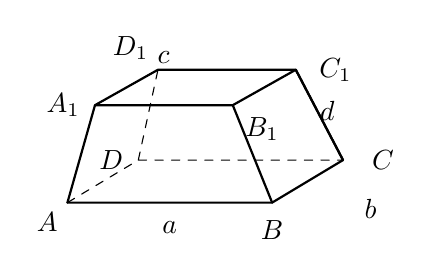
\begin{tikzpicture}[x=1cm,y=.75cm,line cap=round,line join=round]
  \coordinate (A) at (0,0);\coordinate (B) at (2.6,0);\coordinate (C) at (3.5,.72);\coordinate (D) at (.9,.72);
  \coordinate (A1) at (.35,1.65);\coordinate (B1) at (2.1,1.65);\coordinate (C1) at (2.9,2.25);\coordinate (D1) at (1.15,2.25);
  \draw[thick] (A)--(B)--(C)--(C1)--(B1)--(A1)--(D1)--(C1);
  \draw[thick] (A)--(A1) (B)--(B1) (C)--(C1);
  \draw[dashed] (A)--(D) (D)--(C) (D)--(D1);
  % 尺寸标签：置于对应棱外侧，避开棱线与顶点标签
  \node at (1.30,-.42) {$a$};   % 下底面前棱 AB
  \node at (3.85,-.10) {$b$};   % 下底面右棱 BC 外侧
  \node at (1.22,2.46) {$c$};   % 上底面宽 A1B1（顶面后棱之上）
  \node at (3.30,1.55) {$d$};   % 上底面深 B1C1 外侧
  \node[below left] at (A) {$A$};\node[below=3pt] at (B) {$B$};\node[right=7pt] at (C) {$C$};\node[left=2pt] at (D) {$D$};
  \node[left=2pt] at (A1) {$A_1$};\node[below right=1pt] at (B1) {$B_1$};\node[right=5pt] at (C1) {$C_1$};\node[above left] at (D1) {$D_1$};
\end{tikzpicture}
\end{center}
\nopagebreak[4]
\end{question}
\begin{question}
\gkti{19}数列 \(\{a_n\}\) 由下列条件确定：\(x_1=a>0\)，
\nopagebreak[4]
\[
x_{n+1}=\frac12\left(x_n+\frac{a}{x_n}\right),\qquad n\in\mathbb N.
\]

（1） 证明：对 \(n\geqslant2\)，总有 \(x_n\geqslant\sqrt a\)；

（2） 证明：对 \(n\geqslant2\)，总有 \(x_n\geqslant x_{n+1}\)。

\end{question}
\begin{question}
\gkti{20}在研究并行计算的基本算法时，有以下简单模型问题：用计算机求 \(n\) 个不同的数 \(v_1,v_2,\ldots,v_n\) 的和
\nopagebreak[4]
\[
\sum_{i=1}^n v_i=v_1+v_2+\cdots+v_n,
\]
计算开始前，\(n\) 个数存贮在 \(n\) 台由网络连接的计算机中，每台机器存一个数。计算开始后，在一个单位时间内，每台机器至多到一台其他机器中读数据，并与自己原有数据相加得到新的数据，各台机器可同时完成上述工作。为了用尽可能少的单位时间，即可完成计算，方法可用下表表示（表中「1 读」「1 果」分别表示第一单位时间的被读机号与结果，其余类推（表头为排印缩写，原页为「第一单位时间·被读机号」等全称）。）：

\begin{center}
\begingroup\setlength{\tabcolsep}{4pt}
\begin{tabular}{cccccccc}
\toprule
机器号 & 初始 & 1 读 & 1 果 & 2 读 & 2 果 & 3 读 & 3 果 \\
\midrule
1 & \(v_1\) & 2 & \(v_1+v_2\) &  &  &  &  \\
2 & \(v_2\) & 1 & \(v_2+v_1\) &  &  &  &  \\
\bottomrule
\end{tabular}
\endgroup
\end{center}

（1） 当 \(n=4\) 时，至少需要多少个单位时间可完成计算？把你设计的方法填入下表：

\begin{center}
\begingroup\setlength{\tabcolsep}{4pt}
\begin{tabular}{cccccccc}
\toprule
机器号 & 初始 & 1 读 & 1 果 & 2 读 & 2 果 & 3 读 & 3 果 \\
\midrule
1 & \(v_1\) &  &  &  &  &  &  \\
2 & \(v_2\) &  &  &  &  &  &  \\
3 & \(v_3\) &  &  &  &  &  &  \\
4 & \(v_4\) &  &  &  &  &  &  \\
\bottomrule
\end{tabular}
\endgroup
\end{center}

（2） 当 \(n=128\) 时，要使所有机器都得到 \(\sum_{i=1}^{n}v_i\)，至少需要多少个单位时间可完成计算？（结论不要求证明。）

\end{question}
\begin{question}
\gkti{21}已知 \(O(0,0)\)，\(B(1,0)\)，\(C(b,c)\) 是 \(\triangle OBC\) 的三个顶点。

（1） 写出 \(\triangle OBC\) 的重心 \(G\)、外心 \(F\)、垂心 \(H\) 的坐标，并证明 \(G,F,H\) 三点共线；

（2） 当直线 \(FH\) 与 \(OB\) 平行时，求顶点 \(C\) 的轨迹。

\end{question}
\begin{question}
\gkti{22}已知 \(f(x)\) 是定义在 \(\mathbb R\) 上的不恒为零的函数，且对于任意的 \(a,b\in\mathbb R\) 都满足
\nopagebreak[4]
\[
f(a\cdot b)=a f(b)+b f(a).
\]

（1） 求 \(f(0),f(1)\) 的值；

（2） 判断 \(f(x)\) 的奇偶性，并证明你的结论；

（3） 若 \(f(2)=2\)，\(u_n=f(2^n)\)（\(n\in\mathbb N\)），求证 \(u_{n+1}>u_n\)（\(n\in\mathbb N\)）。

\end{question}